%\documentclass[10pt]{beamer}
%\usefonttheme[onlylarge]{structurebold}

\documentclass[handout]{beamer}
\usefonttheme[onlylarge]{structurebold}
  \usepackage{pgfpages}
\mode<handout>
\pgfpagesuselayout{4 on 1}[letterpaper,border shrink=5mm]

\hypersetup{
  bookmarks = false,
  colorlinks,
  citecolor = red,
  linkcolor=blue,
  pdfpagemode=none,
  pdfstartview={Fit},
  pdftitle={},
  pdfauthor={Michael E. Waugh},
  pdfkeywords={} }
  \setbeamertemplate{navigation symbols}{}

\mode<presentation> {
  \usetheme{boxes}
  % or ...

  \setbeamercovered{transparent}
  % or whatever (possibly just delete it)
}

\setbeamertemplate{itemize subitem}[circle]
\setbeamerfont{frametitle}{size= \large}
\setbeamerfont{ framesubtitle }{size = \footnotesize}
\setbeamertemplate{frametitle}
{
\medskip
\smallskip
{\textsf{\underline{\insertframetitle\phantom{))))))))}}}}}


\usepackage[english]{babel}
\usepackage{wasysym}

\addfootbox{}{\hspace{3cm}\tiny {National Income: Where It Comes From---Economics of Global Business, Revised: \today}}%

\title[NYU Stern] % (optional, use only with long paper titles)
{\Large National Income \\ \medskip \Large Where It Comes From}

\author[Michael Waugh] % (optional, use only with lots of authors)
{\bf{\Large}}%

\date[] % (optional)

\subject{Talks}

\begin{document}
%
%

\begin{frame}
  \titlepage
\end{frame}

%%%%%%%%%%%%%%%%%%%%%%%%%%%%%%%%%%%%%%%%%%%%%%%%%%%%%%%%%%%%%%%%%%%%%%%%%%%%%%%%%%%%%%%%%%%%%%%%%%
%%%%%%%%%%%%%%%%%%%%%%%%%%%%%%%%%%%%%%%%%%%%%%%%%%%%%%%%%%%%%%%%%%%%%%%%%%%%%%%%%%%%%%%%%%%%%%%%%%
%
%
\begin{frame}[t]
\frametitle{The Plan for the Week}
\begin{itemize}
\item A static, model economy\ldots
\bigskip
\item Supply Side
\begin{itemize}
\medskip
\item A production function
\medskip
\item How factor markets operate (supply, demand, price)
\medskip
\item Determination of output/income and the distribution of income.
\end{itemize}
\bigskip
\item (Next Week) Demand Side
\begin{itemize}
\medskip
\item Demand for consumption
\medskip
\item Demand for investment
\end{itemize}
\bigskip
\item Please read Chapter 3 (Mankiw).
\end{itemize}
\bigskip
\end{frame}

%%%%%%%%%%%%%%%%%%%%%%%%%%%%%%%%%%%%%%%%%%%%%%%%%%%%%%%%%%%%%%%%%%%%%%%%%%%%%%%%%%%%%%%%%%%%%%%%%
%%%%%%%%%%%%%%%%%%%%%%%%%%%%%%%%%%%%%%%%%%%%%%%%%%%%%%%%%%%%%%%%%%%%%%%%%%%%%%%%%%%%%%%%%%%%%%%%%

\begin{frame}[t]
\frametitle{Factors of Production}
\begin{itemize}
\item $K  =$ Capital. \\
\medskip
Tools, machines, and structures used in production
\bigskip
\item $L  =$ Labor. \\
\medskip
The physical and mental efforts of workers
\bigskip
\item Today, the supplies of capital and labor are fixed (i.e. not changing or exogenous):
\begin{eqnarray*}
K = \bar K \ \ \ \ \mbox{and} \ \ \ \ \ L = \bar L
\end{eqnarray*}
\begin{itemize}
\medskip
\item Future classes, $K$ and $L$ will evolve over time.
\end{itemize}
\end{itemize}
\end{frame}

%%%%%%%%%%%%%%%%%%%%%%%%%%%%%%%%%%%%%%%%%%%%%%%%%%%%%%%%%%%%%%%%%%%%%%%%%%%%%%%%%%%%%%%%%%%%%%%%%
%%%%%%%%%%%%%%%%%%%%%%%%%%%%%%%%%%%%%%%%%%%%%%%%%%%%%%%%%%%%%%%%%%%%%%%%%%%%%%%%%%%%%%%%%%%%%%%%%


\begin{frame}[t]
\frametitle{Production Function}
\begin{itemize}
\item Idea: Describe how much output or GDP ($Y$) the economy can produce from $K$ units of capital and $L$ units of labor.
\bigskip
\item Reflects the economy's level of technology.
\bigskip
\item Mathematical version:
\begin{eqnarray*}
Y = \mbox{F}(K,L)
\end{eqnarray*}
\vspace{-.5cm}
\begin{itemize}
\item $Y = $ output (GDP)
\medskip
\item $K = $ capital, $L = $ labor
\end{itemize}
\bigskip
%\item Cobb-Douglas version
%\begin{eqnarray*}
%Y = A K^{\alpha}L^{\beta}.
%\end{eqnarray*}
\end{itemize}
\end{frame}

%%%%%%%%%%%%%%%%%%%%%%%%%%%%%%%%%%%%%%%%%%%%%%%%%%%%%%%%%%%%%%%%%%%%%%%%%%%%%%%%%%%%%%%%%%%%%%%%%
%%%%%%%%%%%%%%%%%%%%%%%%%%%%%%%%%%%%%%%%%%%%%%%%%%%%%%%%%%%%%%%%%%%%%%%%%%%%%%%%%%%%%%%%%%%%%%%%%


\begin{frame}[t]
\frametitle{Production Function Properties}
\begin{itemize}
\item More inputs lead to more output
\begin{itemize}
\medskip
\item Positive marginal products of capital and labor
\end{itemize}
\bigskip
\item Diminishing marginal products
\begin{itemize}
\medskip
\item If we double \textcolor{red}{only one input}, this leads to a \textcolor{red}{less than} double additional output.
\end{itemize}
\bigskip
\item Constant returns to scale
\begin{itemize}
\medskip
\item If we double \textcolor{red}{both inputs}, this \textcolor{red}{doubles} output.
\end{itemize}
\end{itemize}
\bigskip
\end{frame}

%%%%%%%%%%%%%%%%%%%%%%%%%%%%%%%%%%%%%%%%%%%%%%%%%%%%%%%%%%%%%%%%%%%%%%%%%%%%%%%%%%%%%%%%%%%%%%%%%
%%%%%%%%%%%%%%%%%%%%%%%%%%%%%%%%%%%%%%%%%%%%%%%%%%%%%%%%%%%%%%%%%%%%%%%%%%%%%%%%%%%%%%%%%%%%%%%%%

\begin{frame}[t]
\frametitle{Diminishing Marginal Product to Labor}
\begin{center}
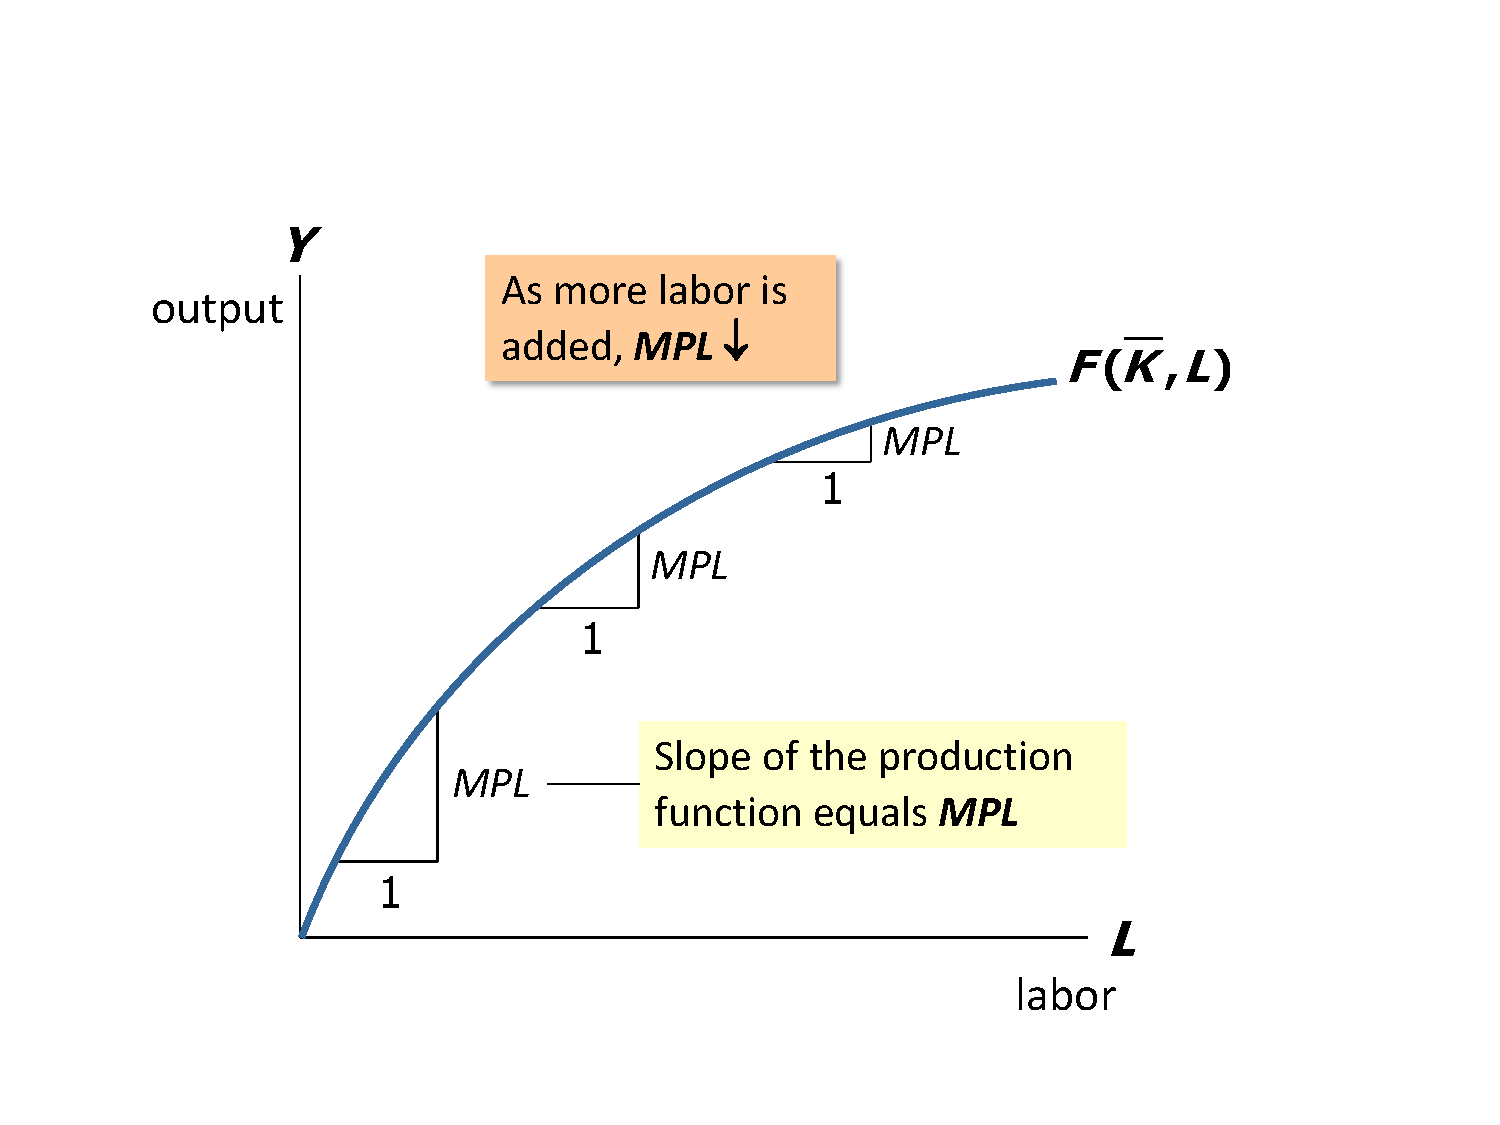
\includegraphics[height=3.1in,width=4.25in]{../Figures/mpl_labor.pdf}
\end{center}
\end{frame}

%%%%%%%%%%%%%%%%%%%%%%%%%%%%%%%%%%%%%%%%%%%%%%%%%%%%%%%%%%%%%%%%%%%%%%%%%%%%%%%%%%%%%%%%%%%%%%%%%
%%%%%%%%%%%%%%%%%%%%%%%%%%%%%%%%%%%%%%%%%%%%%%%%%%%%%%%%%%%%%%%%%%%%%%%%%%%%%%%%%%%%%%%%%%%%%%%%%


\begin{frame}[t]
\frametitle{How Are Factor Demands Determined?}
\begin{itemize}
\item Think of a typical firm in the economy which is competitive.
\begin{itemize}
\medskip
\item What does competitive mean here?
\end{itemize}
\bigskip
\item The goal of the firm is to maximize profits:
\begin{eqnarray*}
\mbox{Profit} = \max_{K,L} \left\{ \ P \times F(K,L) - W \times L - R \times K \ \right\}
\end{eqnarray*}
\item where
\begin{itemize}
\medskip
\item P = product price
\medskip
\item W = wage rate, \ R = rental rate of capital.
\end{itemize}
\end{itemize}
\end{frame}

%%%%%%%%%%%%%%%%%%%%%%%%%%%%%%%%%%%%%%%%%%%%%%%%%%%%%%%%%%%%%%%%%%%%%%%%%%%%%%%%%%%%%%%%%%%%%%%%%
%%%%%%%%%%%%%%%%%%%%%%%%%%%%%%%%%%%%%%%%%%%%%%%%%%%%%%%%%%%%%%%%%%%%%%%%%%%%%%%%%%%%%%%%%%%%%%%%%

\begin{frame}[t]
\frametitle{The Marginal Product of Labor \#1}
\begin{itemize}
\item Marginal Product of Labor $=$ extra amount of output (Y) the firm gets from using one extra unit of labor.
\bigskip
\item Mathematically:
\begin{eqnarray*}
\mbox{MPL}(L+1) = F(\bar K,L+1) - F(\bar K,L)
\end{eqnarray*}
\bigskip
\item What shape does the MPL have given what we assumed about the production function?
\bigskip
\medskip
\item \small Mathematics note: Formally, this is the partial derivative of production function. If our production function is Cobb-Douglas, what is the marginal product of labor?
\end{itemize}
\end{frame}

%%%%%%%%%%%%%%%%%%%%%%%%%%%%%%%%%%%%%%%%%%%%%%%%%%%%%%%%%%%%%%%%%%%%%%%%%%%%%%%%%%%%%%%%%%%%%%%%%
%%%%%%%%%%%%%%%%%%%%%%%%%%%%%%%%%%%%%%%%%%%%%%%%%%%%%%%%%%%%%%%%%%%%%%%%%%%%%%%%%%%%%%%%%%%%%%%%%

\begin{frame}[t]
\frametitle{The Marginal Product of Labor \#2}
\begin{itemize}
\item Basic Idea: Profit maximization dictates the firm hires labor up to the point the change in revenue from adding one more worker is just offset by its cost. Why?
\bigskip
\item Mathematically:
\begin{eqnarray*}
\Delta \mbox{Profit} &=& \Delta \mbox{Revenue} - \Delta \mbox{Cost}, \\
\\
\normalsize &=& P \times \mbox{MPL} - W
\end{eqnarray*}
Profit maximization implies:
\begin{eqnarray*}
P \times \mbox{MPL} = W \ \ \ \ \mbox{or} \ \ \ \ \mbox{MPL} = \frac{W}{P}
\end{eqnarray*}
\medskip
\item \textbf{Key:} Real wage (W/P) reflects the marginal product of labor.
\end{itemize}
\end{frame}

%%%%%%%%%%%%%%%%%%%%%%%%%%%%%%%%%%%%%%%%%%%%%%%%%%%%%%%%%%%%%%%%%%%%%%%%%%%%%%%%%%%%%%%%%%%%%%%%%
%%%%%%%%%%%%%%%%%%%%%%%%%%%%%%%%%%%%%%%%%%%%%%%%%%%%%%%%%%%%%%%%%%%%%%%%%%%%%%%%%%%%%%%%%%%%%%%%%

\begin{frame}[t]
\frametitle{Labor Demand}
\begin{center}
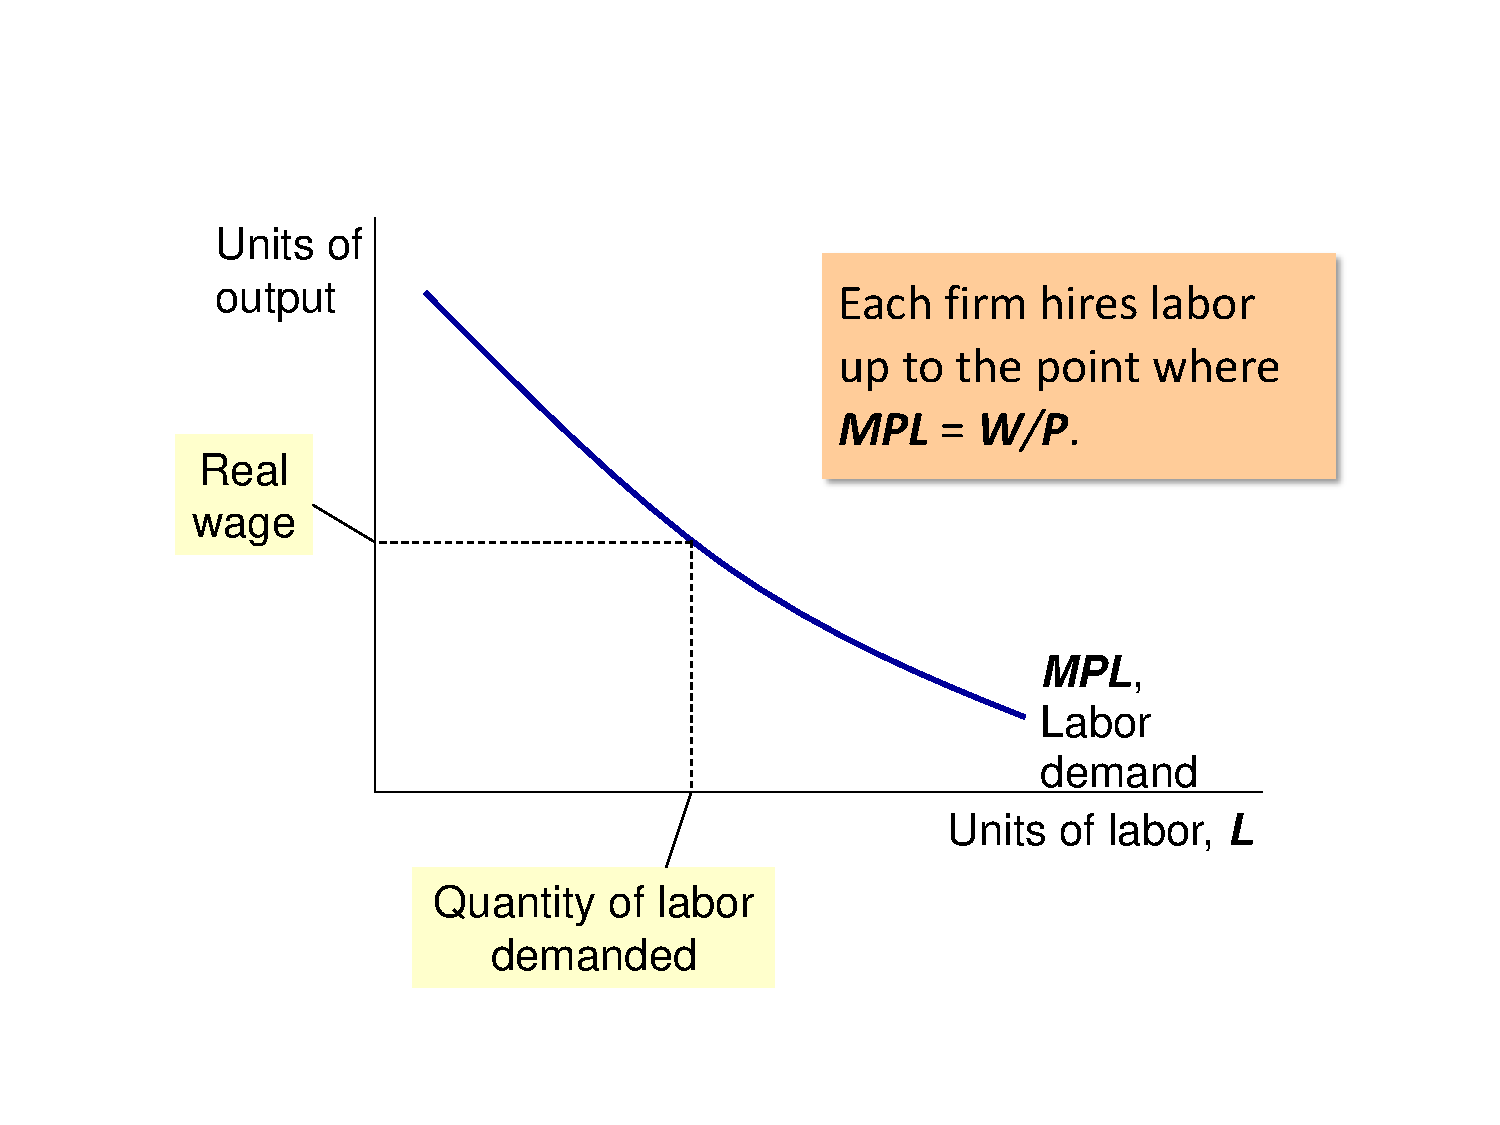
\includegraphics[height=3.1in,width=4.25in]{../Figures/labor_demand1.pdf}
\end{center}
\end{frame}

\begin{frame}[t]
\frametitle{Labor Market Equilibrium}
\begin{center}
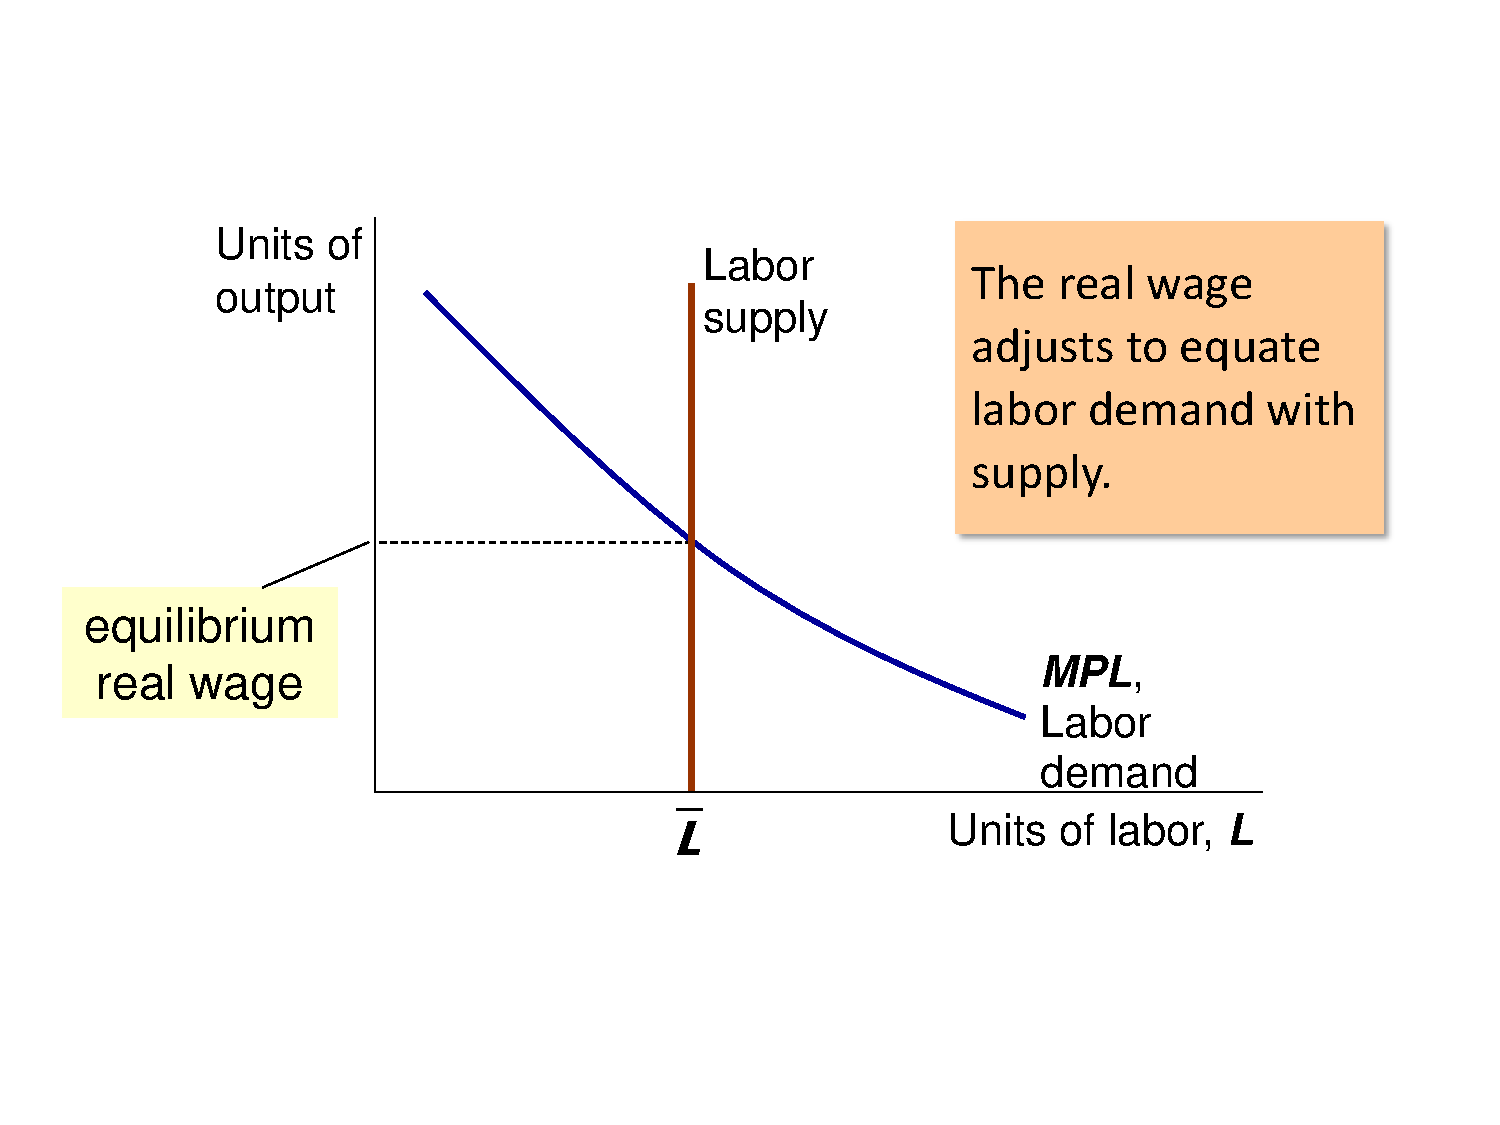
\includegraphics[height=3.1in,width=4.25in]{../Figures/labor_demand2.pdf}
\end{center}
\end{frame}

%%%%%%%%%%%%%%%%%%%%%%%%%%%%%%%%%%%%%%%%%%%%%%%%%%%%%%%%%%%%%%%%%%%%%%%%%%%%%%%%%%%%%%%%%%%%%%%%%
%%%%%%%%%%%%%%%%%%%%%%%%%%%%%%%%%%%%%%%%%%%%%%%%%%%%%%%%%%%%%%%%%%%%%%%%%%%%%%%%%%%%%%%%%%%%%%%%%

\begin{frame}[t]
\frametitle{Wages and Labor productivity, US Data}
\bigskip
\begin{itemize}
\item Theory predicts real wages (W/P) depend on labor productivity (Y/L).
\end{itemize}
\begin{center}
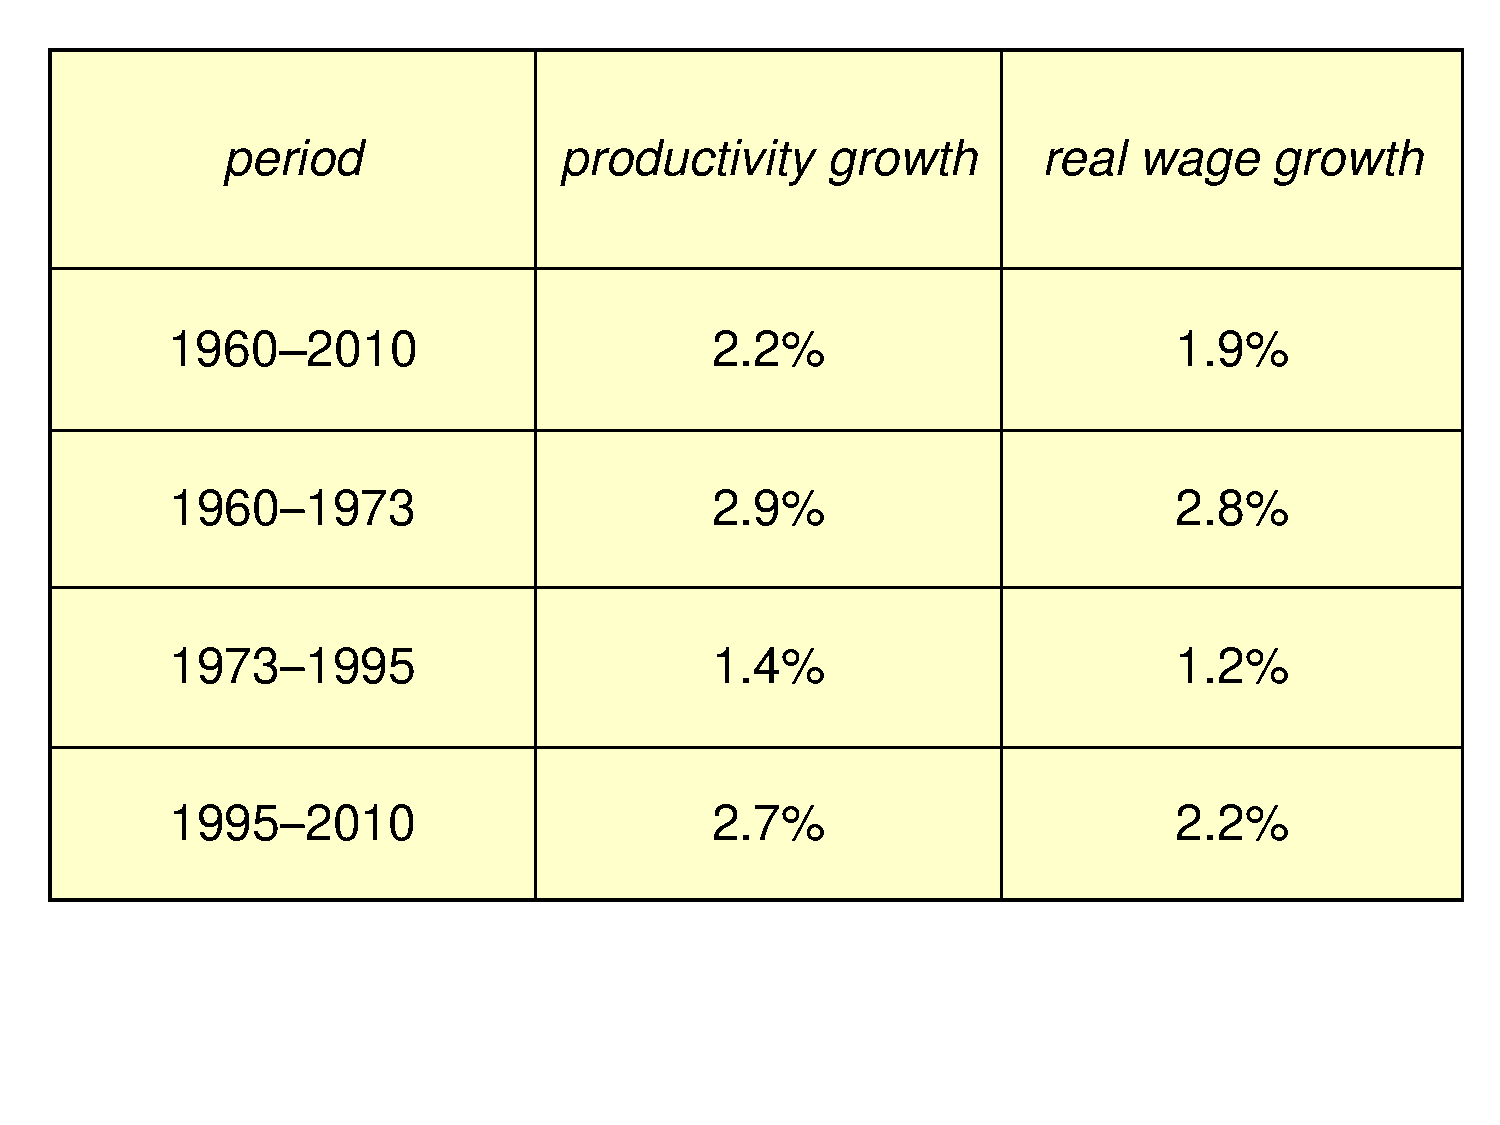
\includegraphics[height=2.5in,width=3.75in]{../Figures/wage_data.pdf}
\end{center}
\end{frame}

%%%%%%%%%%%%%%%%%%%%%%%%%%%%%%%%%%%%%%%%%%%%%%%%%%%%%%%%%%%%%%%%%%%%%%%%%%%%%%%%%%%%%%%%%%%%%%%%%
%%%%%%%%%%%%%%%%%%%%%%%%%%%%%%%%%%%%%%%%%%%%%%%%%%%%%%%%%%%%%%%%%%%%%%%%%%%%%%%%%%%%%%%%%%%%%%%%%

\begin{frame}[t]
\frametitle{The Marginal Product of Capital}
\begin{itemize}
\item Previous logic also implies that the marginal product of capital (MPK) $=$ real rental rate of capital (R/P).
\begin{itemize}
\bigskip
\item Diminishing marginal returns to capital implies $\mbox{MPK}\downarrow$ as $K\uparrow$.
\bigskip
\item Profit maximization dictates the firm hires capital up to the point the change in revenue ($P \times \mbox{MPK}$) from adding one unit of capital is just offset by its cost.
\bigskip
\item The solution implies
\begin{eqnarray*}
P \times \mbox{MPK} = R \ \ \ \ \mbox{or} \ \ \ \ \mbox{MPK} = \frac{R}{P}
\end{eqnarray*}
\end{itemize}
\end{itemize}
\end{frame}

%%%%%%%%%%%%%%%%%%%%%%%%%%%%%%%%%%%%%%%%%%%%%%%%%%%%%%%%%%%%%%%%%%%%%%%%%%%%%%%%%%%%%%%%%%%%%%%%%
%%%%%%%%%%%%%%%%%%%%%%%%%%%%%%%%%%%%%%%%%%%%%%%%%%%%%%%%%%%%%%%%%%%%%%%%%%%%%%%%%%%%%%%%%%%%%%%%%

\begin{frame}[t]
\frametitle{Capital Market Equilibrium}
\begin{center}
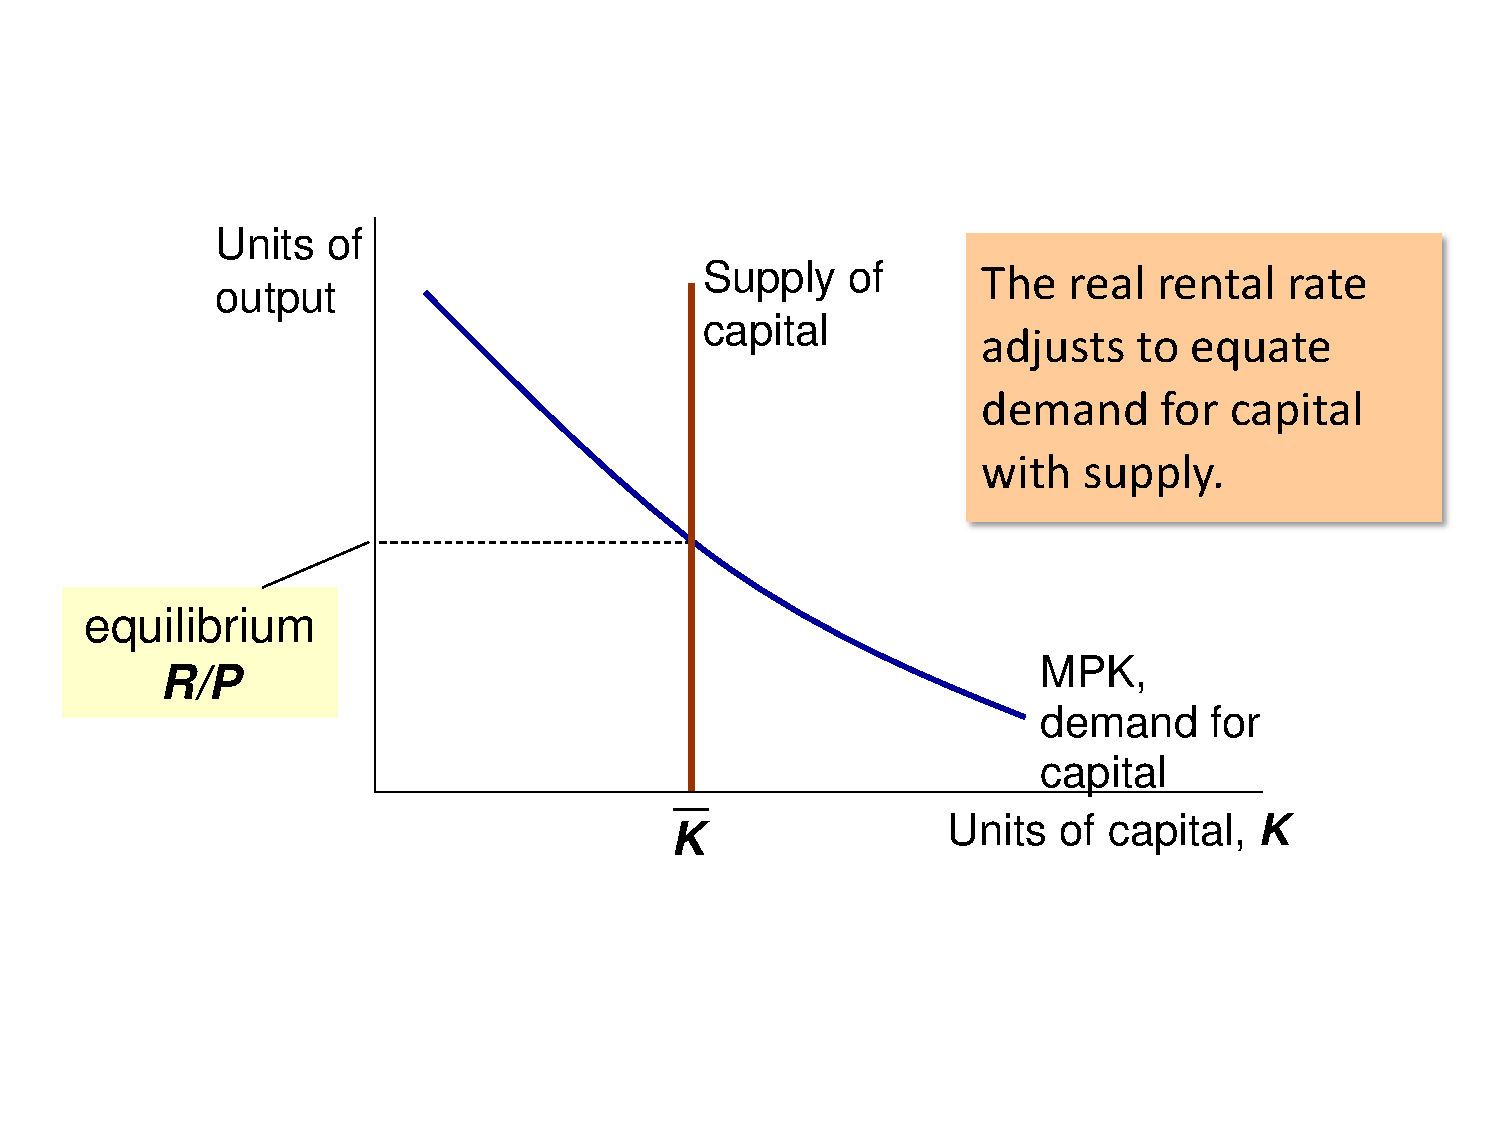
\includegraphics[height=3.1in,width=4.25in]{../Figures/capital_demand.pdf}
\end{center}
\end{frame}

%%%%%%%%%%%%%%%%%%%%%%%%%%%%%%%%%%%%%%%%%%%%%%%%%%%%%%%%%%%%%%%%%%%%%%%%%%%%%%%%%%%%%%%%%%%%%%%%%
%%%%%%%%%%%%%%%%%%%%%%%%%%%%%%%%%%%%%%%%%%%%%%%%%%%%%%%%%%%%%%%%%%%%%%%%%%%%%%%%%%%%%%%%%%%%%%%%%
\begin{frame}[t]
\frametitle{Cobb-Douglas Production Function}
\begin{itemize}
\item Cobb-Douglas production function
\begin{eqnarray*}
Y = \mbox{F}(K,L) = A K^\alpha L^{1-\alpha}
\end{eqnarray*}
\begin{itemize}
\item where $\alpha$ control's share of income to labor and capital.
\medskip
\item $A = $ total factor productivity, i.e. the level of technology.
\end{itemize}
\bigskip
\item What type of returns to scale does this have? Does it have diminishing and positive marginal products?
\end{itemize}
\end{frame}

%%%%%%%%%%%%%%%%%%%%%%%%%%%%%%%%%%%%%%%%%%%%%%%%%%%%%%%%%%%%%%%%%%%%%%%%%%%%%%%%%%%%%%%%%%%%%%%%%
%%%%%%%%%%%%%%%%%%%%%%%%%%%%%%%%%%%%%%%%%%%%%%%%%%%%%%%%%%%%%%%%%%%%%%%%%%%%%%%%%%%%%%%%%%%%%%%%%
\begin{frame}[t]
\frametitle{Cobb-Douglas Marginal Products}
\begin{itemize}
\item Cobb-Douglas production function
\begin{eqnarray*}
Y = \mbox{F}(K,L) = A K^\alpha L^{1-\alpha}
\end{eqnarray*}
\begin{itemize}
\item Marginal Product of Labor (MPL)
\begin{eqnarray*}
\mbox{MPL} = \frac{\partial \mbox{F}(K,L)}{L} &=& (1-\alpha)A K^\alpha L^{-\alpha}\\
\\
 &=& (1-\alpha) \frac{Y}{L}
\end{eqnarray*}
\medskip
\item Marginal Product of Capital (MPK)
\begin{eqnarray*}
\mbox{MPK} = \frac{\partial \mbox{F}(K,L)}{K} &=&\alpha A K^{\alpha-1} L^{1-\alpha}\\
\\
 &=& \alpha \frac{Y}{K}
\end{eqnarray*}
\end{itemize}
\end{itemize}
\end{frame}


%%%%%%%%%%%%%%%%%%%%%%%%%%%%%%%%%%%%%%%%%%%%%%%%%%%%%%%%%%%%%%%%%%%%%%%%%%%%%%%%%%%%%%%%%%%%%%%%%
%%%%%%%%%%%%%%%%%%%%%%%%%%%%%%%%%%%%%%%%%%%%%%%%%%%%%%%%%%%%%%%%%%%%%%%%%%%%%%%%%%%%%%%%%%%%%%%%%

\begin{frame}[t]
\frametitle{Practice Questions\ldots}
\begin{itemize}
\item[1.] Does an increase in TFP change the real rental rate of capital?
\bigskip
\item[2.] Labor force participation is falling in the US, is this good or bad for the owners of capital?
\bigskip
\item[3.] Burma is currently a closed economy and does not allow the free flow of capital (in or out).\\
\medskip
If Burma's current rental rate of capital is $R^B/P > R^*/P$ (the world equilibrium rental rate of capital), how would you expect capital to flow in or out of Burma.
\medskip
\item[4.] How would wages in Burma be affected?
\end{itemize}
\end{frame}


%%%%%%%%%%%%%%%%%%%%%%%%%%%%%%%%%%%%%%%%%%%%%%%%%%%%%%%%%%%%%%%%%%%%%%%%%%%%%%%%%%%%%%%%%%%%%%%%%
%%%%%%%%%%%%%%%%%%%%%%%%%%%%%%%%%%%%%%%%%%%%%%%%%%%%%%%%%%%%%%%%%%%%%%%%%%%%%%%%%%%%%%%%%%%%%%%%%

\begin{frame}[t]
\frametitle{How is Income Distributed in the Economy? I}
\begin{itemize}
\item Income inequality is a hot topic. This model can speak to some of the current issues.
\bigskip
\item Income payments to labor and capital:
\begin{itemize}
\medskip
\item Labor income $= \frac{W}{P}\bar L \ = \mbox{MPL}\times \bar L$
\medskip
\item Capital income $= \frac{R}{P}\bar K \ = \mbox{MPK}\times \bar K$
\end{itemize}
\bigskip
\item Total (Real) GDP $=$ payments to income, so \ldots
\begin{eqnarray*}
\bar Y = \mbox{MPL}\times \bar L + \mbox{MPK}\times \bar K
\end{eqnarray*}
\end{itemize}
\end{frame}

%%%%%%%%%%%%%%%%%%%%%%%%%%%%%%%%%%%%%%%%%%%%%%%%%%%%%%%%%%%%%%%%%%%%%%%%%%%%%%%%%%%%%%%%%%%%%%%%%
%%%%%%%%%%%%%%%%%%%%%%%%%%%%%%%%%%%%%%%%%%%%%%%%%%%%%%%%%%%%%%%%%%%%%%%%%%%%%%%%%%%%%%%%%%%%%%%%%

\begin{frame}[t]
\frametitle{How is Income Distributed in the Economy? II}
\begin{itemize}
\item Total (Real) GDP $=$ payments to income, so \ldots
\begin{eqnarray*}
\bar Y = \mbox{MPL}\times \bar L + \mbox{MPK}\times \bar K
\end{eqnarray*}
\bigskip
\item Plugging in the marginal products, from previous slide:
\begin{eqnarray*}
\bar Y& =& (1-\alpha)\frac{\bar Y}{\bar L}\times \bar L + \alpha \frac{\bar Y}{\bar K}\times \bar K \\
\\
& =& (1-\alpha)\bar Y + \alpha \bar Y
\end{eqnarray*}
\item Which implies Labor's Share of income is $(1-\alpha)$!
\end{itemize}
\end{frame}

%%%%%%%%%%%%%%%%%%%%%%%%%%%%%%%%%%%%%%%%%%%%%%%%%%%%%%%%%%%%%%%%%%%%%%%%%%%%%%%%%%%%%%%%%%%%%%%%%%
%%%%%%%%%%%%%%%%%%%%%%%%%%%%%%%%%%%%%%%%%%%%%%%%%%%%%%%%%%%%%%%%%%%%%%%%%%%%%%%%%%%%%%%%%%%%%%%%%%

\begin{frame}[t]
\frametitle{A Static, Model Economy}
\bigskip
\begin{itemize}
\item Supply Side
\begin{itemize}
\medskip
\item A production function $\Large {\color{red}\checkmark}$
\medskip
\item How factor markets operate (supply, demand, price) $\Large {\color{red}\checkmark}$
\medskip
\item Determination of output/income and the distribution of income $\Large {\color{red}\checkmark}$
\end{itemize}
\end{itemize}
\bigskip
\end{frame}






\end{document}
